\section{Критерий существования стационарного режима марковской цепи}

\textbf{Автор:} Миндиярова Рената, Б-01-009

\subsection{Определение марковской цепи}
     В схеме Бернулли с $\Omega = \{\omega: {\omega = (x_1, ... x_n), x_i=0,1}\}$   вероятность $p(\omega)$ каждого исхода $\omega$ задавалась формулой  
\begin{equation} \label{mindiiarova_eq_1} 
p(\omega) = p(x_1)...p (x_n)
\end{equation}
 где $p(x)=p^xq^{1-x}$. При этом условии случайные величины $ \xi_1, ...,\xi_n$ с $\xi_n(\omega)=x_i$ оказывались независимыми и одинаково распределенными с 
\begin{center}
$P(\xi_1 = x) = ... = P(\xi_n = x) = p(x), x = 0,1 $
\end{center}

Если вместо (\ref{mindiiarova_eq_1}) положить 
\begin{center}
$p(\omega) = p_1 (x_1)...p_n (x_n)$,
\end{center}

 где $p_i(x)=p^x_i(1-p_i)^{1-x}$, $0\leq	p_i\leq	1$, то тогда случайные величины $ \xi_1, ...,\xi_n$ также будут \textit{независимыми}, но уже, вообще говоря, \textit{разнораспределенными}:
\begin{center}
$P(\xi_1 = x) = p_1 (x), ..., P(\xi_n = x) = p_n (x)$
\end{center}

Рассмотрим теперь одно обобщение этих систем, приводящее к \textit{зависимым} случайным величинам, образующим так называемую цепь Маркова.


Будем предполагать, что
\begin{center}
$\Omega = \{ \omega: \omega = (x_0, x_1, ..., x_n), x_i \in X \} $,
\end{center}
где X - некоторое конечное множество. Пусть заданы также неотрицательные функции $p_0(x), p_1(x,y), ..., p_n(x,y)$ такие, что 

\begin{equation} \label{mindiiarova_eq_2} 
\sum\limits_{x \in X} p_0 (x) = 1,\sum\limits_{y \in X} p_k (x, y) = 1, k = 1, ..., n; y \in X
\end{equation}

Для каждого исхода $\omega = (x_0, x_1, ..., x_n)$ положим
\begin{equation} \label{mindiiarova_eq_3} 
p(\omega) = p_0 (x_0) p_1 (x_0, x_1)...p_n (x_{n-1}, x_n)
\end{equation}

Нетрудно проверить, что $\sum\limits_{\omega \in \Omega} p(\omega) = 1$ и,
следовательно, набор этих чисел p($\omega)$ вместе с пространством $\Omega$ и системой всех его подмножеств опредяляет некоторую вероятностную модель, которую принято называть \textit{моделью испытаний, связанных в цепь Маркова}.


Введем в рассмотрение случайные величины $\xi_0, \xi_1, ...,\xi_n$ с 
    $\xi_i(\omega)=x_i$. Простой подсчет показывает, что
\begin{equation} \label{mindiiarova_eq_4} 
P(\xi_0 = a) = p_0(a), P(\xi_0 = a_0, ..., \xi_k = a_k ) = p_0(a) p_1(a_0, a_1)...p_1(a_{k-1}, a_k)
\end{equation}
Из (4) следует простое свойство условных вероятностей:
\begin{equation} \label{mindiiarova_eq_5} 
P \{ \xi_{k+1} = a_{k+1} | \xi_{k} = a_{k}, ..., \xi_{0} = a_{0} \} = P \{ \xi_{k+1} = a_{k+1} | \xi_{k} = a_{k}\}
\end{equation}

\begin{center}
(в предположении  $ P (\xi_k = a_k, ..., \xi_0 = a_0) > 0)$
\end{center}

Пусть $\mathscr{D}^\xi_k = \mathscr{D}_{\xi_0, ..., \xi_k} $ --разбиение, порожденное величинами  $ \xi_0, \xi_1, ...,\xi_k$, и $\mathscr{B}^\xi_k=\alpha(\mathscr{D}^\xi_k) $.


Из (\ref{mindiiarova_eq_5}) следует, что

\begin{equation} \label{mindiiarova_eq_6} 
P \{ \xi_{k+1} = a_{k+1} | \mathscr{B}^{\xi}_k \} = P \{ \xi_{k+1} = a_{k+1} | \xi_k\}
\end{equation}
или
\begin{equation} \label{mindiiarova_eq_7} 
P \{ \xi_{k+1} = a_{k+1} |\xi_0, ...,\xi_k \} = P \{ \xi_{k+1} = a_{k+1} | \xi_k\}
\end{equation}

Если воспользоваться очевидным равенством
\begin{equation} \label{mindiiarova_eq_8} 
P \text(AB|C) = P \text(A|BC) P \text(B|C)
\end{equation}

то из (\ref{mindiiarova_eq_6}) получаем, что
\begin{equation} \label{mindiiarova_eq_9} 
P \{ \xi_n = a_n, ..., \xi_{k+1} = a_{k+1} | \mathscr{B}^{\xi}_k \} = P \{ \xi_n = a_n, ..., \xi_{k+1} = a_{k+1} | \xi_k\}
\end{equation}
или  
\begin{equation} \label{mindiiarova_eq_10} 
P \{ \xi_n = a_n, ..., \xi_{k+1} = a_{k+1} |\xi_0, ...,\xi_k  \} = P \{ \xi_n = a_n, ..., \xi_{k+1} = a_{k+1} | \xi_k\}
\end{equation}

Это равенство допускает следующую наглядную интерпретацию. Будем трактовать
$\xi_k$ как положение частицы в "настоящем",  $(\xi_0, ...,\xi_{k-1})$ - в "прошлом" и   $(\xi_{k+1}, ...,\xi_n)$ - в "будущем". Тогда (\ref{mindiiarova_eq_10}) означает, что при фиксированных "прошлом" $(\xi_0, ...,\xi_{k-1})$ и "настоящем"  $\xi_k$ и не зависит от того, каким способом частица попала в точку $\xi_k$, т.е не зависит от "прошлого" $(\xi_0, ...,\xi_{k-1})$.


Пусть $\text{Б}$ = $\{\xi_n = a_n, ..., \xi_{k+1} = a_{k+1}\} $, $H = \{\xi_k=a_k\}$, $ \text{П} =  \{\xi_{k-1} = a_{k-1}, ..., \xi_0 = a_0\}$.
Тогда из (\ref{mindiiarova_eq_10}) следует, что
\begin{center}
$P($Б$|$НП$) = P($Б$|$Н$)$
\end{center} 
откуда следует, что
\begin{equation} \label{mindiiarova_eq_11} 
P(\text{БП|Н}) = P(\text{Б|Н})P(\text{П|Н})
\end{equation}
Иначе говоря, из (\ref{mindiiarova_eq_6}) следует, что при фиксированном "настоящем" Н, "будущее" Б и "прошлое" П оказываются независимыми. Нетрудно показать, что справедливо и обратное: из выполнения (\ref{mindiiarova_eq_11}) для любого $k = 0, 1, ..., n-1$
следует выполнение свойства (\ref{mindiiarova_eq_6}) для всякого $k = 0, 1, ..., n-1$.


Свойство независимости "будущего" и "прошлого", или, что то же, независимость "будущего" от "прошлого" при фиксированном "настоящем" принято называть \textit{марковским свойством}, а соответсвующую последовательность случайных величин   $(\xi_{0}, ...,\xi_n)$ - \textit{марковской цепью}.


Таким образом, если вероятности $p(\omega)$ элементарных событий задаются формулой (\ref{mindiiarova_eq_3}) то последовательность  $\xi = (\xi_0, ...,\xi_n)$ c $\xi_i(\omega)=x_i$, будет образовывать марковскую цепь.


В этой связи понятно следующее:


\begin{definition}
Пусть $(\Omega,  \mathscr{A}, P)$ - некоторое (конечное) вероятностное пространство и $\xi = (\xi_0, ...,\xi_n)$ - последовательность случайных величин со значениями в (конечном) множестве X. Если выполнено условие (\ref{mindiiarova_eq_6}), то последовательность $\xi = (\xi_0, ...,\xi_n)$ называется (конечной) \textit{марковской цепью}.


Множество X называется \textit{фазовым пространством}или \textit{пространством состояний} цепи. Набор вероятностей $(p_n(x)))$, $x\in X$, c $(p_0(x))) = P(\xi_0=x)$ называют \textit{начальным распределением}, а матрицу 
$
\begin{Vmatrix}
    p_k (x,y)
\end{Vmatrix}
$
, $x,y \in X$, c  $(p_k(x, y))) = P(\xi_k=y|\xi_{k-1}=x)$ - \textit{матрицей переходных вероятностей} (из состояний x в состояние y) в момент $k = 1, ..., n$.


В том случае, когда переходные вероятности $p_k(x, y))$ не зависят от 
$k,p_k(x, y)) = p(x, y))$, последовательность $\xi = (\xi_0, ...,\xi_n)$ называется однородной марковской цепью с матрицей переходных вероятностей 
$\begin{Vmatrix}
    p(x,y)
\end{Vmatrix}$
\end{definition}

Заметим, что матрица 
$\begin{Vmatrix}
    p(x,y)
\end{Vmatrix}$
является \textit{стохастической}: ее элементы неотрицательны и сумма элементов любой ее строки равна единице,  $\sum\limits_{y}p(x, y) = 1 , x \in X$.

Будем считать, что фазовое пространство X состоит из конечного множества целочисленных точек $(X = \{0, 1,... , N\}, X = \{0, \pm1, ..., \pm{N}\}$и т.д.) и обозначать $p_i=p_0(i)$ и $p_{ij} = p(i, j)$. а 


Понятно, что свойства однородных марковских цепей полностью определяются начальными распределниями $p_i$ и переходными вероятностями $p_{i j}$. В конкретных случаях для описания эволюции цепи вместо явного выписывания матрицы $\begin{Vmatrix}
    p(x_i,y_j)
\end{Vmatrix}$ используют (ориентированный) граф, вершинами которого являются состояния их X, а стрелка 

\begin{figure}[h]
\centering
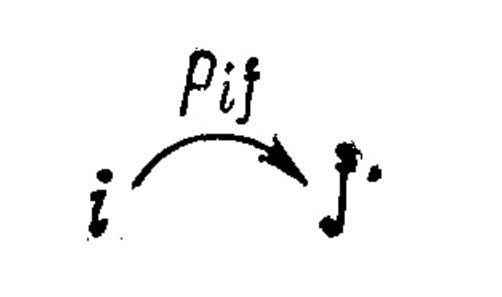
\includegraphics[width=0.2\linewidth]{mindiiarova_pic_1.jpg}
\label{fig:mpr}
\end{figure}


идущая из состояния i в состояние j и с числом $p_{ij}$ над ней, показывает, что из точки i возможен переход в точку j с вероятностью $p_{ij}$. В том случае, когда $p_{ij} = 0$, соответствующая стрелка не проводится.

\subsection{Эргодическая теорема}

Следующая теорема описывает широкий класс марковских цепей, обладающих так называем свойством \textit{эргодичности}: пределы  $\pi =  \lim_{n}p_{ij}^{(n)} $ не только существуют, не зависят от i, образуют распределение вероятностей ($\pi_j \geq 0, \sum\limits_{j}\pi_j = 1$, но и таковы, что $\pi_j > 0$ при всех j (такие распределения $\pi_j$ называются  \textit{эргодическими}).



\begin{theorem}

Пусть $\mathbb{P}$ =  
$\begin{Vmatrix}
    p_{ij}
\end{Vmatrix}  $
- \textit{матрица переходных вероятностей марковской цепи с конечным множеством состояний $X = \{1, 2, ..., N\}$}.

\begin{enumerate}[label=\alph*)]
\item  Если \textit{найдется $n_0$ такое, что} 
\begin{equation} \label{mindiiarova_eq_12} 
    \min_{i,j}p_{ij}^{(n_0)}>0,
\end{equation}
то существуют числа $\pi_1, ..., \pi_N$ такие, что
\begin{equation} \label{mindiiarova_eq_13} 
    \pi_j > 0,  \sum\limits_{j}\pi_j = 1
\end{equation}
и для любого $i \in X$
\begin{equation} \label{mindiiarova_eq_14} 
    p_{ij}^{(n)} \rightarrow \pi_j ,  n \rightarrow \infty.
\end{equation}

\item Обратно, если сущесвуют числа $\pi_1, ..., \pi_N$, удовлетворяющие условиям (\ref{mindiiarova_eq_13}) и (\ref{mindiiarova_eq_14}), то найдется $n_0$ такое, что выполненое условие (\ref{mindiiarova_eq_12}).

\item Числа  $(\pi_1, ..., \pi_N)$ удовлетворяют системе уравнений
\begin{equation} \label{mindiiarova_eq_15} 
    \pi_j = \sum\limits_{\alpha}\pi_{\alpha}p_{\alpha j}, j = 1, ..., N
\end{equation}
\end{enumerate}

\end{theorem}


\begin{proof}

a) Обозначим
\begin{equation} \label{mindiiarova_eq_16} 
      m_j^{(n)} = \min_{i}p_{ij}^{(n)}, M_j^{(n)} = \max_{i}p_{ij}^{(n)}
\end{equation}
Поскольку
\begin{equation} \label{mindiiarova_eq_17} 
      p_{ij}^{(n+1)} =  \sum\limits_{\alpha}p_{\alpha j}p_{\alpha j}^{(n)}
\end{equation}
то
\begin{equation}\label{mindiiarova_eq_18} 
      m_{j}^{(n+1)} =  \min_{i}p_{ij}^{(n+1)} =  \min_{i}\sum\limits_{\alpha}p_{i \alpha}p_{\alpha j}^{(n)} \geq \min_{i}\sum\limits_{\alpha}p_{i \alpha}\min_{\alpha}p_{\alpha j}^{(n)} = m_j^{(n)},
\end{equation}
откуда $m_j^{(n)} \leq m_j^{(n+1)}$ и аналогично $M_j^{(n)} \geq M_j^{(n+1)}$. Поэтому для доказательства утверждения (14) достаточно показать, что 
\begin{equation} \label{mindiiarova_eq_19} 
     M_j^{(n)} - m_j^{(n)} \rightarrow 0, 
     n \rightarrow \infty, j =1, ..., N.
\end{equation}
Пусть $\varepsilon = \min_{i, j}p_{ij}^{(n_0)} > 0$. Тогда

\begin{multline} \label{mindiiarova_eq_20} 
     p_{i j}^{(n_0+n)} = \sum\limits_{\alpha}p_{i \alpha}^{(n_0)}p_{\alpha j}^{(n)} =\sum\limits_{\alpha}(p_{i \alpha}^{(n_0)} - \varepsilon p_{\alpha j}^{(n))})p_{\alpha j}^{(n)} +\varepsilon\sum\limits_{\alpha}p_{j \alpha}^{(n)}p_{\alpha j}^{(n)} = \
     \\
   = \sum\limits_{\alpha}(p_{i \alpha}^{(n_0)} - \varepsilon p_{\alpha j}^{(n))})p_{\alpha j}^{(n)} + \varepsilon p^{(2n)}_{j j}.
\end{multline}
Но $p_{i \alpha}^{(n_0)} - \varepsilon p_{\alpha j}^{(n))} \geq 0$, поэтому 
\begin{equation} \label{mindiiarova_eq_21} 
     p_{ij}^{(n+n_0)} \geq m_j^{(n)} \cdot \sum\limits_{\alpha}(p_{i \alpha}^{(n_0)} - \varepsilon p_{\alpha j}^{(n))}) + \varepsilon p^{(2n)}_{i j} = m_j^{(n)}(1-\varepsilon)+\varepsilon p^{(2n)}_{j j},
\end{equation}
и, значит, 
\begin{equation} \label{mindiiarova_eq_22} 
     m_j^{(n_0+n)} \geq m_j^{(n)}(1-\varepsilon)+\varepsilon p^{(2n)}_{i j}
\end{equation}
Аналогичным образом
\begin{equation} \label{mindiiarova_eq_23} 
     M_j^{(n_0+n)} \leq M_j^{(n)}(1-\varepsilon)+\varepsilon p^{(2n)}_{i j}
\end{equation}
Объединяя эти неравенства, получаем
\begin{equation} \label{mindiiarova_eq_24} 
     M_j^{(n_0+n)} - m_j^{(n_0+n)} \leq (M_j^{(n)} - m_j^{(n)}) \cdot(1-\varepsilon)
\end{equation}
и, следовательно,
\begin{equation}\label{mindiiarova_eq_25} 
     M_j^{(kn_0+n)} - m_j^{(kn_0+n)} \leq (M_j^{(n)} - m_j^{(n)}) \cdot(1-\varepsilon)^k \rightarrow  0, k  \rightarrow \infty.
\end{equation}
Итак, по некоторой подпоследовательности \{$n_\beta$\} $M_j^{(n_\beta)} - m_j^{(n_\beta)}  \rightarrow 0, n_\beta \rightarrow \infty$. Но разность $M_j^{(n)} - m_j^{(n)}$ монотонна по n, а значит, $M_j^{(n)} - m_j^{(n)}  \rightarrow 0, n_\beta \rightarrow \infty$.
Если обозначить $\pi_j = \lim_{n} m_j^{(n)}$, то из полученных оценок следует, что для  $n \geq n_0$
\begin{equation} \label{mindiiarova_eq_26} 
     |p_{i j}^{(n)} - \pi_j| \leq M_j^{(n)} - m_j^{(n)} \leq (1-\varepsilon)^{(n/n_0) - 1},
\end{equation}
т.е сходимость $p_{i j}^{(n)}$ к предельным значеним $\pi_j$ происходит с геометрической скорость.

Ясно также, что $m_j^{(n)} \geq  m_j^{(n_0)} \geq \varepsilon > 0, n \geq n_0$, и, значит, $\pi_j >0$.


b) Условие (\ref{mindiiarova_eq_12}) непосредственно следует из (\ref{mindiiarova_eq_14}), посколько число состояний конечно и $\pi_j >0$.


c) Уравнение (\ref{mindiiarova_eq_15}) вытекают из (\ref{mindiiarova_eq_14}) и (\ref{mindiiarova_eq_17}).

\end{proof}

\subsection{Стационарное распределение вероятностей}
 Система уравнений (\ref{mindiiarova_eq_15}) играет большую роль в теории марковских цепей.
 Всякое ее неотрицательное решение $(\pi_1, ..., \pi_N)$, удовлетворяющее условию $\sum\limits_{\alpha}\pi_{\alpha} = 1$, принято называть \textit{стационарным} или \textit{инвариантным}, распределением вероятностей для марковской цепи с матрицей вероятностей 
 $
 \begin{Vmatrix}
    p_{ij}
\end{Vmatrix}.$
Объяснение состоит в следующем.


Возьмем распределение $(\pi_1, ..., \pi_N)$ в качестве начального, $p_j=\pi_j$. Тогда 
\begin{equation} \label{trivial}
     p_j^{(n)} = \sum\limits_{\alpha}\pi_{\alpha}p_{\alpha j}= \pi_j
\end{equation}
и вообще $p_j^{(n)} =\pi_j$. Иначе говоря, если в качестве начального распределения взять  $(\pi_1, ..., \pi_N)$, то это распределение не будет изменяться со временем,т.е для любого k
\begin{equation} \label{trivial}
     P(\xi_k=j) =  P(\xi_0=j), j = 1, ..., N.
\end{equation}
Более того, с таким начальным распределением марковская цепь $\xi = (\xi, \Pi,\mathbb{P})$ будет \textit{стационарной}: совместное распределение вектора $(\xi_k, ..., \xi_{k+l})$ не зависит от k для любого l (предполагается, что $k+l\leq n$)


Условие (\ref{mindiiarova_eq_12}) гарантирует как существование пределов $\pi_j = \lim_{n}p_{i j }^{(n)}$, не зависящих от i, так и существование эргодического распределения, т.е распределение с $\pi_j>0$. Распределение $(\pi_1, ..., \pi_N)$ оказывается также и \textit{стационарным} распределением. Покажем сейчас, что набор $(\pi_1, ..., \pi_N)$ является \textit{единственным} стационарным распределением.


В самом деле, пусть $(\tilde{\pi_1}, ..., \tilde{\pi_N})$ -- еще одно стационарное распределение. Тогда
\begin{equation} \label{trivial}
     \tilde{\pi_j} = \sum\limits_{\alpha}\tilde{\pi}_{\alpha}p_{\alpha j} = 
     ... = \sum\limits_{\alpha}\tilde{\pi}_{\alpha}p_{\alpha j}^{(n)}
\end{equation}
и поскольку $p_{i j}^{(n)} \rightarrow  \pi_j$, то
\begin{equation} \label{trivial}
     \tilde{\pi}_j= \sum\limits_{\alpha}(\tilde{\pi}_{\alpha} \cdot p_{i j})=\pi_j.
\end{equation}
В связи с этими результатами возникают интересные и важные вопросы о достаточных, необходимых, а также необходимых и достаточных условиях, при которых: (A)  \textit{существуют} пределы $\pi_j=\lim_{n}p_{i j}^{(n)}$, не зависящие от i; (B) пределы $(\pi_1, ..., \pi_N)$ образуют  \textit{распределение вероятностей}; (C) пределы $(\pi_1, ..., \pi_N)$ образуют \textit{эргодическое} распределение вероятностей; (D) \textit{сущесвтвует} и при том \textit{единственное} стационарное распределение вероятностей.
\subsection{Дополнение}
\begin{definition}
Рассмотрим какой-нибудь (конечный) неупорядоченный набор $\tau = [t_1, ..., t_n]$ различных индексов $t_i in T, n \geq 1$ и пусть $\mathbb{P_{\tau}}$ — вероятностная мера на ($\mathbb{R^{\tau}}, \mathscr{B}(\mathbb{R^{\tau}}) $).  Будем говорить, что семейство вероятностных мер {$\mathbb{P_{\tau}}$}, где $\tau$ пробегает множество всех конечных неупорядоченныхнаборов, согласовано, если для любых наборов  $\tau = [t_1, ..., t_n]$ и $\sigma =[s_1, ..., s_k]$  таких, что $\sigma in \tau$ и для любого $B \in  \mathscr{B}(\mathbb{R^{\sigma}})$

 \begin{equation} \label{trivial}
\mathbb{P_{\sigma}}\{(x_{s_1}, ..., x_{s_k}):(x_{s_1}, ..., x_{s_k}) \in B\} = \mathbb{P_{\tau}}\{(x_{t_1}, ..., x_{t_k}):(x_{s_1}, ..., x_{s_k}) \in B\}
\end{equation}
\end{definition}


\begin{theorem}[Колмогорова о продолжении меры в ($\mathbb{R^{T}}, \mathscr{B}(\mathbb{R^{T}}) $)]
Пусть  $\mathbb{P_{\tau}}$ — семейство согласованных вероятностных мер на $\mathbb{R^{\tau}}, \mathscr{B}(\mathbb{R^{\tau}}) $.Тогда существует, и притом единственная, вероятностная мера $\mathbb{P}$ на $\mathbb{R^{T}}, \mathscr{B}(\mathbb{R^{T}}) $, такая что $\mathbb{P}\{x \in \mathbb{R^{T}} : (x_{t_1}, ..., x_{t_k}) \in B\}  = \mathbb{P}_{[t_1, ..., t_n](B)}$ для
всех неупорядоченных наборов $\tau = [t_1, ..., t_n]$ различных индексов $t_i \in T$ и $B \in  \mathscr{B}$ (другими словами,$ \mathbb{P_{\tau}} = (\pi_{(T\rightarrow \tau)})_{*}\mathbb{P}$)
\end{theorem}

\begin{proof}
1. Отметим прежде всего, что если T не более чем счётно, то по предыдущей
теорема такая мера существует и единственна. Действительно, зафиксировав нумерацию $T = \{t_1, t_2, ...\}$ и воспользовавшись изоморфизмом $\mathbb{R^{T}} \cong \mathbb{R^{{\infty}}}$, по теореме  можем построить меру на $\mathbb{R^{T}}$, используя $\mathbb{P}_{n} = \mathbb{P}_{\{t_1,...,t_n\}}$. Построенная мера $\mathbb{P}$ будет удовлетворять равенству $ \mathbb{P_{\tau}} = (\pi_{(T\rightarrow \tau)})_{*}\mathbb{P}$ для
$\tau = \{t_1, ..., t_n\}, n \geq 1 $, и будет единственной с этим свойством. Чтобы доказать это свойство для произвольного конечного $\tau$, выберем $n$ так, что $\tau \in \{t_1, ..., t_n\} = \tau' $. Тогда
\begin{equation}
    \mathbb{P_{\tau}} = (\pi_{\tau' \rightarrow \tau})_{*} \mathbb{P}_{n} =  (\pi_{\tau' \rightarrow \tau})_{*}(\pi_{T \rightarrow \tau'})_{*}  \mathbb{P} = (\pi_{\tau' \rightarrow \tau})(\pi_{T \rightarrow \tau'})_{*}  \mathbb{P} = (\pi_{T \rightarrow \tau})_{*}  \mathbb{P}
\end{equation}
2. Пусть теперь T произвольно. Рассмотрим $M  \in  \mathscr{B}(\mathbb{R^{T}})$ По предложению $M \in \mathscr{B}_s$, т.е. $M = \pi^{-1}_{(T \rightarrow S)}(M_s)$ для некоторого не более чем счётного S и $M  \in  \mathscr{B}(\mathbb{R^{S}})$.. Применив теорему к множеству S и мерам $\mathbb{P}_{\tau}, \tau \in S$, получим меру $ \mathbb{P}_{s}$. Теперь положим
\begin{equation}
     \mathbb{P}(M) :=   \mathbb{P}_{s}(M_{s}) 
\end{equation}
Покажем, что так определённая мера $ \mathbb{P}$ будет корректно определена и $\sigma$ аддитивна. (Требуемая в теореме единственность будет вытекать из единственности мер $ \mathbb{P}_{s}$.)
Если $M \in \mathscr{B}_{s_1} $ и $M \in \mathscr{B}_{s_2} $, то $M \in \mathscr{B}_{s_1 \cup s_2}$, поэтому при проверке корректности можно
ограничиться случаем $S \in S'$. Итак, $M = \pi^{-1}_{(T \rightarrow S)}(M_s) = \pi^{-1}_{(T \rightarrow S')}(M'_s).$ Но тогда
\begin{equation}
   \pi^{-1}_{(T \rightarrow S')}(M'_s) =  \pi^{-1}_{(T \rightarrow S)}(M_s) =  \pi^{-1}_{(T \rightarrow S')} \pi^{-1}_{(S' \rightarrow S)} (M_s) 
\end{equation}
Поскольку $\pi_{(T \rightarrow S')}$ сюръективно, отсюда следует, что $M'_{S} = \pi^{-1}_{(S' \rightarrow S)} (M_s) $. . Но тогда корректность
сводится к равенству 
\begin{equation}
    \mathbb{P}_{S'}(\pi^{-1}_{(S' \rightarrow S)} (Y)) =  \mathbb{P}_{S}(Y)
\end{equation}
для $Y = M_s$. Его истинность при всех $Y \in \mathscr{B}(\mathbb{R^{S}}) $
следует из того факта, что обе части 35 как функции от Y удовлетворяют условиям теоремы для множества $S$ и мер $ \mathbb{P}_{\tau}, \tau \in S$, а значит, совпадают.
\end{proof}
 


\begin{remark} Исходное семейство вероятностных мер \{$\mathbb{P}_{\tau}$\} предполагалось заданным для всех неупорядоченных наборов $\tau = [t_1,...,t_n] $ различных индексов. Однако можно было начать и с семейства вероятностных мер $\mathbb{P}_{\tau}$, где $\tau$ пробегает семейство всех {\it упорядоченных} наборов  $\tau = (t_1,...,t_n)$ различных индексов. В таком случае для справедливости только что доказанной теоремы Колмагорова необходимо добавить дополнительное условие согласованности, а именно
\begin{equation}
\mathbb{P}_{(t_1, ...t_n)}(A_{t_1}\times...\times A_{t_n}) = \mathbb{P}_{(t_{i_1}, ...t_{i_n})}(A_{t_{i_1}}\times...\times A_{t_{i_n}})
\end{equation}
где $(i_1, ..., i_n)$ есть перестановка чисел $(1,...,n)$, а $A_{t_i} \in \mathfrak{B}(\mathbb{R}_{t_i})$. Нетрудно видеть, что это условие является необходимым для существования меры $\mathbb{P}$, о которой говорится в условии теоремы Колмогорова . Детали мы оставляем читателю, отметим лишь, что 36 есть частный случай равенства $\mathbb{P}_{(t_1, ...t_n)} = (f_{\sigma})_*{P}_{(t_{\sigma(1)}, ...t_{\sigma(n)})}$, где $f_{\sigma}$ переставляет координаты в $\mathbb{R}^n$ согласно перестановке $\sigma$.
\end{remark}






